\documentclass[acmsmall,10pt]{acmart}%
\settopmatter{printfolios=true,printccs=false,printacmref=false}

%%%%%%%%%%%%%%
%%%%%%%%%%%%%%
%% Template 

%% Conference information
%% Supplied to authors by publisher for camera-ready submission;
%% use defaults for review submission.
\acmConference[PL'17]{ACM SIGPLAN Conference on Programming Languages}{January 01--03, 2017}{New York, NY, USA}
\acmYear{2017}
\acmISBN{} % \acmISBN{978-x-xxxx-xxxx-x/YY/MM}
\acmDOI{} % \acmDOI{10.1145/nnnnnnn.nnnnnnn}
\startPage{1}

%% Copyright information
%% Supplied to authors (based on authors' rights management selection;
%% see authors.acm.org) by publisher for camera-ready submission;
%% use 'none' for review submission.
\setcopyright{none}
%\setcopyright{acmcopyright}
%\setcopyright{acmlicensed}
%\setcopyright{rightsretained}
%\copyrightyear{2017}           %% If different from \acmYear

%% Bibliography style
\bibliographystyle{acmart/ACM-Reference-Format}
%% Citation style
%\citestyle{acmauthoryear}  %% For author/year citations
%\citestyle{acmnumeric}     %% For numeric citations
%\setcitestyle{nosort}      %% With 'acmnumeric', to disable automatic
                            %% sorting of references within a single citation;
                            %% e.g., \cite{Smith99,Carpenter05,Baker12}
                            %% rendered as [14,5,2] rather than [2,5,14].
%\setcitesyle{nocompress}   %% With 'acmnumeric', to disable automatic
                            %% compression of sequential references within a
                            %% single citation;
                            %% e.g., \cite{Baker12,Baker14,Baker16}
                            %% rendered as [2,3,4] rather than [2-4].


%% END TEMPLATE
%%%%%%%%%%%%%%%%%%%%
%%%%%%%%%%%%%%%%%%%%

%%%%%%%%%%%%%%%%%%%%
%%%%%%%%%%%%%%%%%%%%
%
% Our formatting rules and included packages.
%
%% ODER: format ==         = "\mathrel{==}"
%% ODER: format /=         = "\neq "
%
%
\makeatletter
\@ifundefined{lhs2tex.lhs2tex.sty.read}%
  {\@namedef{lhs2tex.lhs2tex.sty.read}{}%
   \newcommand\SkipToFmtEnd{}%
   \newcommand\EndFmtInput{}%
   \long\def\SkipToFmtEnd#1\EndFmtInput{}%
  }\SkipToFmtEnd

\newcommand\ReadOnlyOnce[1]{\@ifundefined{#1}{\@namedef{#1}{}}\SkipToFmtEnd}
\usepackage{amstext}
\usepackage{amssymb}
\usepackage{stmaryrd}
\DeclareFontFamily{OT1}{cmtex}{}
\DeclareFontShape{OT1}{cmtex}{m}{n}
  {<5><6><7><8>cmtex8
   <9>cmtex9
   <10><10.95><12><14.4><17.28><20.74><24.88>cmtex10}{}
\DeclareFontShape{OT1}{cmtex}{m}{it}
  {<-> ssub * cmtt/m/it}{}
\newcommand{\texfamily}{\fontfamily{cmtex}\selectfont}
\DeclareFontShape{OT1}{cmtt}{bx}{n}
  {<5><6><7><8>cmtt8
   <9>cmbtt9
   <10><10.95><12><14.4><17.28><20.74><24.88>cmbtt10}{}
\DeclareFontShape{OT1}{cmtex}{bx}{n}
  {<-> ssub * cmtt/bx/n}{}
\newcommand{\tex}[1]{\text{\texfamily#1}}	% NEU

\newcommand{\Sp}{\hskip.33334em\relax}


\newcommand{\Conid}[1]{\mathit{#1}}
\newcommand{\Varid}[1]{\mathit{#1}}
\newcommand{\anonymous}{\kern0.06em \vbox{\hrule\@width.5em}}
\newcommand{\plus}{\mathbin{+\!\!\!+}}
\newcommand{\bind}{\mathbin{>\!\!\!>\mkern-6.7mu=}}
\newcommand{\rbind}{\mathbin{=\mkern-6.7mu<\!\!\!<}}% suggested by Neil Mitchell
\newcommand{\sequ}{\mathbin{>\!\!\!>}}
\renewcommand{\leq}{\leqslant}
\renewcommand{\geq}{\geqslant}
\usepackage{polytable}

%mathindent has to be defined
\@ifundefined{mathindent}%
  {\newdimen\mathindent\mathindent\leftmargini}%
  {}%

\def\resethooks{%
  \global\let\SaveRestoreHook\empty
  \global\let\ColumnHook\empty}
\newcommand*{\savecolumns}[1][default]%
  {\g@addto@macro\SaveRestoreHook{\savecolumns[#1]}}
\newcommand*{\restorecolumns}[1][default]%
  {\g@addto@macro\SaveRestoreHook{\restorecolumns[#1]}}
\newcommand*{\aligncolumn}[2]%
  {\g@addto@macro\ColumnHook{\column{#1}{#2}}}

\resethooks

\newcommand{\onelinecommentchars}{\quad-{}- }
\newcommand{\commentbeginchars}{\enskip\{-}
\newcommand{\commentendchars}{-\}\enskip}

\newcommand{\visiblecomments}{%
  \let\onelinecomment=\onelinecommentchars
  \let\commentbegin=\commentbeginchars
  \let\commentend=\commentendchars}

\newcommand{\invisiblecomments}{%
  \let\onelinecomment=\empty
  \let\commentbegin=\empty
  \let\commentend=\empty}

\visiblecomments

\newlength{\blanklineskip}
\setlength{\blanklineskip}{0.66084ex}

\newcommand{\hsindent}[1]{\quad}% default is fixed indentation
\let\hspre\empty
\let\hspost\empty
\newcommand{\NB}{\textbf{NB}}
\newcommand{\Todo}[1]{$\langle$\textbf{To do:}~#1$\rangle$}

\EndFmtInput
\makeatother
%
%%%%%%%%%%%%%%%%%%%%%%%%%%%%%%
%%
%% Recommended by the ACM ppl
\usepackage{booktabs}
\usepackage{subcaption}

%%%%%%%%%%%%%%%%%%%%%%%%%%%%%%
%%
%% Our packages
\usepackage{xcolor}
\usepackage{booktabs}

%% Cleveref must be the last loaded package
%% since it modifies the cross-ref system.
\usepackage{cleveref}

%%%%%%%%%%%%%%%%%%%%%%%%%%%%%%
%%
%% Our defs

%% More space between rows
\newcommand{\ra}[1]{\renewcommand{\arraystretch}{#1}}

%% Logistic Stuff

\definecolor{C1}{RGB}{0,153,204}
\definecolor{C2}{RGB}{89,0,179}

\newcounter{commentctr}[section]
\setcounter{commentctr}{0}
\renewcommand{\thecommentctr}{%
\arabic{section}.\arabic{commentctr}}

\newcommand{\warnme}[1]{%
{\color{red} \textbf{$[$} #1 \textbf{$]$}}}

\newcommand{\TODO}[1]{%
{\color{purple} \textbf{$[$ TODO: } #1 \textbf{$]$}}}

\newcommand{\tmp}[1]{%
{\color{gray} \textit{#1} }}

\newenvironment{temp}{\bgroup \color{gray} \textit}{\egroup}

\newcommand{\victor}[2][nolabel]{%
{\color{C2} \refstepcounter{commentctr}\label{#1} \textbf{$[$ (\thecommentctr) Victor: } #2 \textbf{$]$}}}

\newcommand{\iris}[2][nolabel]{%
{\color{C1} \refstepcounter{commentctr}\label{#1} \textbf{$[$ (\thecommentctr) Iris: } #2 \textbf{$]$}}}

%% LaTeX stuff

\newenvironment{myhs}{\par\vspace{0.15cm}\begin{minipage}{\textwidth}}{\end{minipage}\vspace{0.15cm}}

%%%%%%%%%%%%%%%%%%%%%%%%%%%%%
%%
%% lhs2TeX Formatting Rules
%%
%% Comment out to use lhs2TeX default formatting.
%%
%%%%%%%%%%%%%%%%%%%%%%%%%%%%%%
%% 
%% Haskell Styling
%%
%% TODO: Figure out spacing!

%% Colors (from duo-tone light syntax)
\definecolor{hsblack}{RGB}{45,32,3}
\definecolor{hsgold1}{RGB}{179,169,149}
\definecolor{hsgold2}{RGB}{177,149,90}
\definecolor{hsgold3}{RGB}{190,106,13}%{192,96,4}%{132,97,19}
\definecolor{hsblue1}{RGB}{173,176,182}
\definecolor{hsblue2}{RGB}{113,142,205}
\definecolor{hsblue3}{RGB}{0,33,132}
\definecolor{hsblue4}{RGB}{97,108,132}
\definecolor{hsblue5}{RGB}{34,50,68}
\definecolor{hsred2}{RGB}{191,121,103}
\definecolor{hsred3}{RGB}{171,72,46}

%% LaTeX Kerning nastiness. By using curly braces to delimit color group,
%% it breaks spacing. The following seems to work:
%%
%% https://tex.stackexchange.com/questions/85033/colored-symbols/85035#85035
%%
\newcommand*{\mathcolor}{}
\def\mathcolor#1#{\mathcoloraux{#1}}
\newcommand*{\mathcoloraux}[3]{%
  \protect\leavevmode
  \begingroup
    \color#1{#2}#3%
  \endgroup
}
\newcommand{\HSKeyword}[1]{\mathcolor{hsgold3}{\textbf{#1}}}
\newcommand{\HSNumeral}[1]{\mathcolor{hsred3}{#1}}
\newcommand{\HSChar}[1]{\mathcolor{hsred2}{#1}}
\newcommand{\HSString}[1]{\mathcolor{hsred2}{#1}}
\newcommand{\HSSpecial}[1]{\mathcolor{hsblue4}{\ensuremath{#1}}}
\newcommand{\HSSym}[1]{\mathcolor{hsblue4}{\ensuremath{#1}}}
\newcommand{\HSCon}[1]{\mathcolor{hsblue3}{#1}}
\newcommand{\HSVar}[1]{\mathcolor{hsblue5}{\mathit{\ensuremath{#1}}}}
\newcommand{\HSComment}[1]{\mathcolor{hsgold2}{\textit{#1}}}


%%% lhs2TeX parser does not recognize '*' 
%%% in kind annotations, it thinks it is a multiplication.


%%

% Easy to typeset Haskell types using the 
% commands from stylish.lhs (if it's defined!)
\newcommand{\HT}[1]{\ifdefined\HSCon\HSCon{#1}\else#1\fi}
\newcommand{\HS}[1]{\ifdefined\HSSym\HSSym{#1}\else#1\fi}
\newcommand{\HV}[1]{\ifdefined\HSVar\HSVar{#1}\else#1\fi}

%%% Datatype Promotion

%%% Usefull Notation



%
%%%%%%%%%%%%%%%%%%%%
%%%%%%%%%%%%%%%%%%%%

\begin{document}

%% Title information
\title[Fractal dimensions in symbolic music data and applications]{Fractal dimensions in symbolic music data and applications}
%\titlenote{with title note}
\subtitle{Pattern discovery and feature analysis}
%\subtitlenote{with subtitle note}


%% Author information
%% Contents and number of authors suppressed with 'anonymous'.
%% Each author should be introduced by \author, followed by
%% \authornote (optional), \orcid (optional), \affiliation, and
%% \email.
%% An author may have multiple affiliations and/or emails; repeat the
%% appropriate command.
%% Many elements are not rendered, but should be provided for metadata
%% extraction tools.

\author{Victor Cacciari Miraldo}
\orcid{nnnn-nnnn-nnnn-nnnn}             %% \orcid is optional
\affiliation{
  \position{PhD candidate}
  \department{Information and Computing Sciences}
  \institution{Utrecht University}
  \streetaddress{Princetonplein, 5}
  \city{Utrecht}
  \state{Utrecht}
  \postcode{3584 CC}
  \country{The Netherlands} 
}
\email{V.CacciariMiraldo@uu.nl}
\author{Iris Yuping Ren}
\orcid{nnnn-nnnn-nnnn-nnnn}             %% \orcid is optional
\affiliation{
  \position{PhD candidate}
  \department{Information and Computing Sciences}
  \institution{Utrecht University}
  \streetaddress{Princetonplein, 5}
  \city{Utrecht}
  \state{Utrecht}
  \postcode{3584 CC}
  \country{The Netherlands} 
}
\email{y.ren@uu.nl}
%% Abstract
%% Note: \begin{abstract}...\end{abstract} environment must come
%% before \maketitle command
\begin{abstract}
  Abstract comes here!
\end{abstract}


%% 2012 ACM Computing Classification System (CSS) concepts
%% Generate at 'http://dl.acm.org/ccs/ccs.cfm'.
\begin{CCSXML}\begingroup\par\noindent\advance\leftskip\mathindent\(
\begin{pboxed}\SaveRestoreHook
\column{B}{@{}>{\hspre}l<{\hspost}@{}}%
\column{E}{@{}>{\hspre}l<{\hspost}@{}}%
\>[B]{}\HSVar{ccs2012}\HSSym{>}{}\<[E]%
\\
\>[B]{}\HSVar{concept}\HSSym{>}{}\<[E]%
\\
\>[B]{}\HSVar{concept\char95 id}\HSSym{>}\HSNumeral{10011007.10011006}\HSSym{\mathbin{\circ}}\HSNumeral{10011008}\HSSym{</}\HSVar{concept\char95 id}\HSSym{>}{}\<[E]%
\\
\>[B]{}\HSVar{concept\char95 desc}\HSSym{>}\HSCon{Software}\;\HSVar{and}\;\HSVar{its}\;\HSVar{engineering}\HSSym{\mathrel{\sim}}\HSCon{General}\;\HSVar{programming}\;\HSVar{languages}\HSSym{</}\HSVar{concept\char95 desc}\HSSym{>}{}\<[E]%
\\
\>[B]{}\HSVar{concept\char95 significance}\HSSym{>}\HSNumeral{500}\HSSym{</}\HSVar{concept\char95 significance}\HSSym{>}{}\<[E]%
\\
\>[B]{}\HSSym{\mathbin{/}}\HSVar{concept}\HSSym{>}{}\<[E]%
\\
\>[B]{}\HSVar{concept}\HSSym{>}{}\<[E]%
\\
\>[B]{}\HSVar{concept\char95 id}\HSSym{>}\HSNumeral{10003456.10003457}\HSSym{\mathbin{\circ}}\HSNumeral{10003521.10003525}\HSSym{</}\HSVar{concept\char95 id}\HSSym{>}{}\<[E]%
\\
\>[B]{}\HSVar{concept\char95 desc}\HSSym{>}\HSCon{Social}\;\HSVar{and}\;\HSVar{professional}\;\HSVar{topics}\HSSym{\mathrel{\sim}}\HSCon{History}\;\HSKeyword{of}\;\HSVar{programming}\;\HSVar{languages}\HSSym{</}\HSVar{concept\char95 desc}\HSSym{>}{}\<[E]%
\\
\>[B]{}\HSVar{concept\char95 significance}\HSSym{>}\HSNumeral{300}\HSSym{</}\HSVar{concept\char95 significance}\HSSym{>}{}\<[E]%
\\
\>[B]{}\HSSym{\mathbin{/}}\HSVar{concept}\HSSym{>}{}\<[E]%
\\
\>[B]{}\HSSym{\mathbin{/}}\HSVar{ccs2012}\HSSym{>}{}\<[E]%
\ColumnHook
\end{pboxed}
\)\par\noindent\endgroup\resethooks
\end{CCSXML}

\ccsdesc[500]{Software and its engineering~General programming languages}
\ccsdesc[300]{Social and professional topics~History of programming languages}
%% End of generated code


%% Keywords
%% comma separated list
\keywords{Music Information Retrieval, Pattern discovery, Haskell}


%% \maketitle
%% Note: \maketitle command must come after title commands, author
%% commands, abstract environment, Computing Classification System
%% environment and commands, and keywords command.
\maketitle

%%%%%%%%%%%%%%%%%%%%%%%%
%%%%%%%%%%%%%%%%%%%%%%%%
%
% Body
%
\section{Introduction}
\label{sec:intro}

%\paragraph{MIR and functional programming}
%DSL
%Type
%Many possibility to explore.

%\paragraph{Musical patterns}
%Automatic musical pattern discovery is hard. 

\paragraph{Hierarchical structures in music}
Music is known to have rich hierarchical structures, ranging from global forms to local phrases, from harmonic progressions to melodic patterns. The hierarchical structures allow us to examine music at different levels of details and time scales. For example, as shown in Figure \ref{fig:egbach}, the original piece on the
top two staffs in
can be summarised by the chords in the third staffs; similarly, in Figure
\ref{fig:egscale}, the patterns
shown on the top staff can be progressively and hierarchically reduced to the
bottom staff. There have been many musical theories on the hierarchical
structure of music, such as the
General Theory of Tonal Music (GTTM) \cite{lerdahl1985generative} and the Schenkerian theory of melodic reduction
\cite{forte1959schenker}.

% \begin{figure}
%    \centering
%     \begin{subfigure}[t]{0.5\textwidth}
%         \centering
%         \includegraphics[width=\linewidth]{eg.png}
%         \caption{Two levels of hierarchies in Bach's Preludium in C
%           major \cite{wiki:bach}: the original piece and the underlying chords.
%           The details in the first two staffs can be summarised into the chords
%           in the third staff. }
%     \end{subfigure}%
%     ~ 
%     \begin{subfigure}[t]{0.5\textwidth}
%         \centering
%         \includegraphics[width=\linewidth]{egscale.png}
%         \caption{Four levels of hierarchies in an artificial example using
%           scales: from the top to the bottom staff, we have different levels of
%           details in different levels of hierarchies. The notes in different
%           levels of hierarchies are specified based on the metrical positions of
%           the notes.  }
%     \end{subfigure}
%     \caption{Examples of hierarchical structures in music}
%   \label{fig:eg}
% \end{figure}

\begin{figure}
  \includegraphics[width=0.7 \linewidth]{eg.png}
  \caption{Two levels of hierarchies in Bach's Preludium in C
          major \cite{wiki:bach}: the original piece and the underlying chords.
          The details in the first two staffs can be summarised into the chords
          in the third staff}
  \label{fig:egbach}
\end{figure}

\begin{figure}
  \includegraphics[width=0.7 \linewidth]{egscale.png}
  \caption{Four levels of hierarchies in an artificial example using
          scales: from the top to the bottom staff, we have different levels of
          details in different levels of hierarchies. The notes in different
          levels of hierarchies are specified based on the metrical positions of
          the notes.}
  \label{fig:egscale}
\end{figure}


%By examining what is the backbone of the piece and  , we can view music from different levels of importance and details.
\paragraph{Hierarchies in fractal geometry}

One tool that could be used to study the hierarchical structure in music is
fractal theory. Fractal geometry is an established area of
mathematics that studies self-similar patterns on different levels of details. The
concept of fractal dimension has been devised to measure the change of contents
across different levels of hierarchies. In the one-dimensional case,
the fractal dimensions takes into account of the line segment lengths at
different scales. For example, as shown in Figure \ref{fig:bc}, empirically, the
fractal dimension can be measured given any contour. Therefore, given a segment
of music, one can also use
the box-counting method to
calculate a parallel of the fractal dimension by looking into the different levels
of details exhibited on different levels of hierarchies in music.

\begin{figure}
  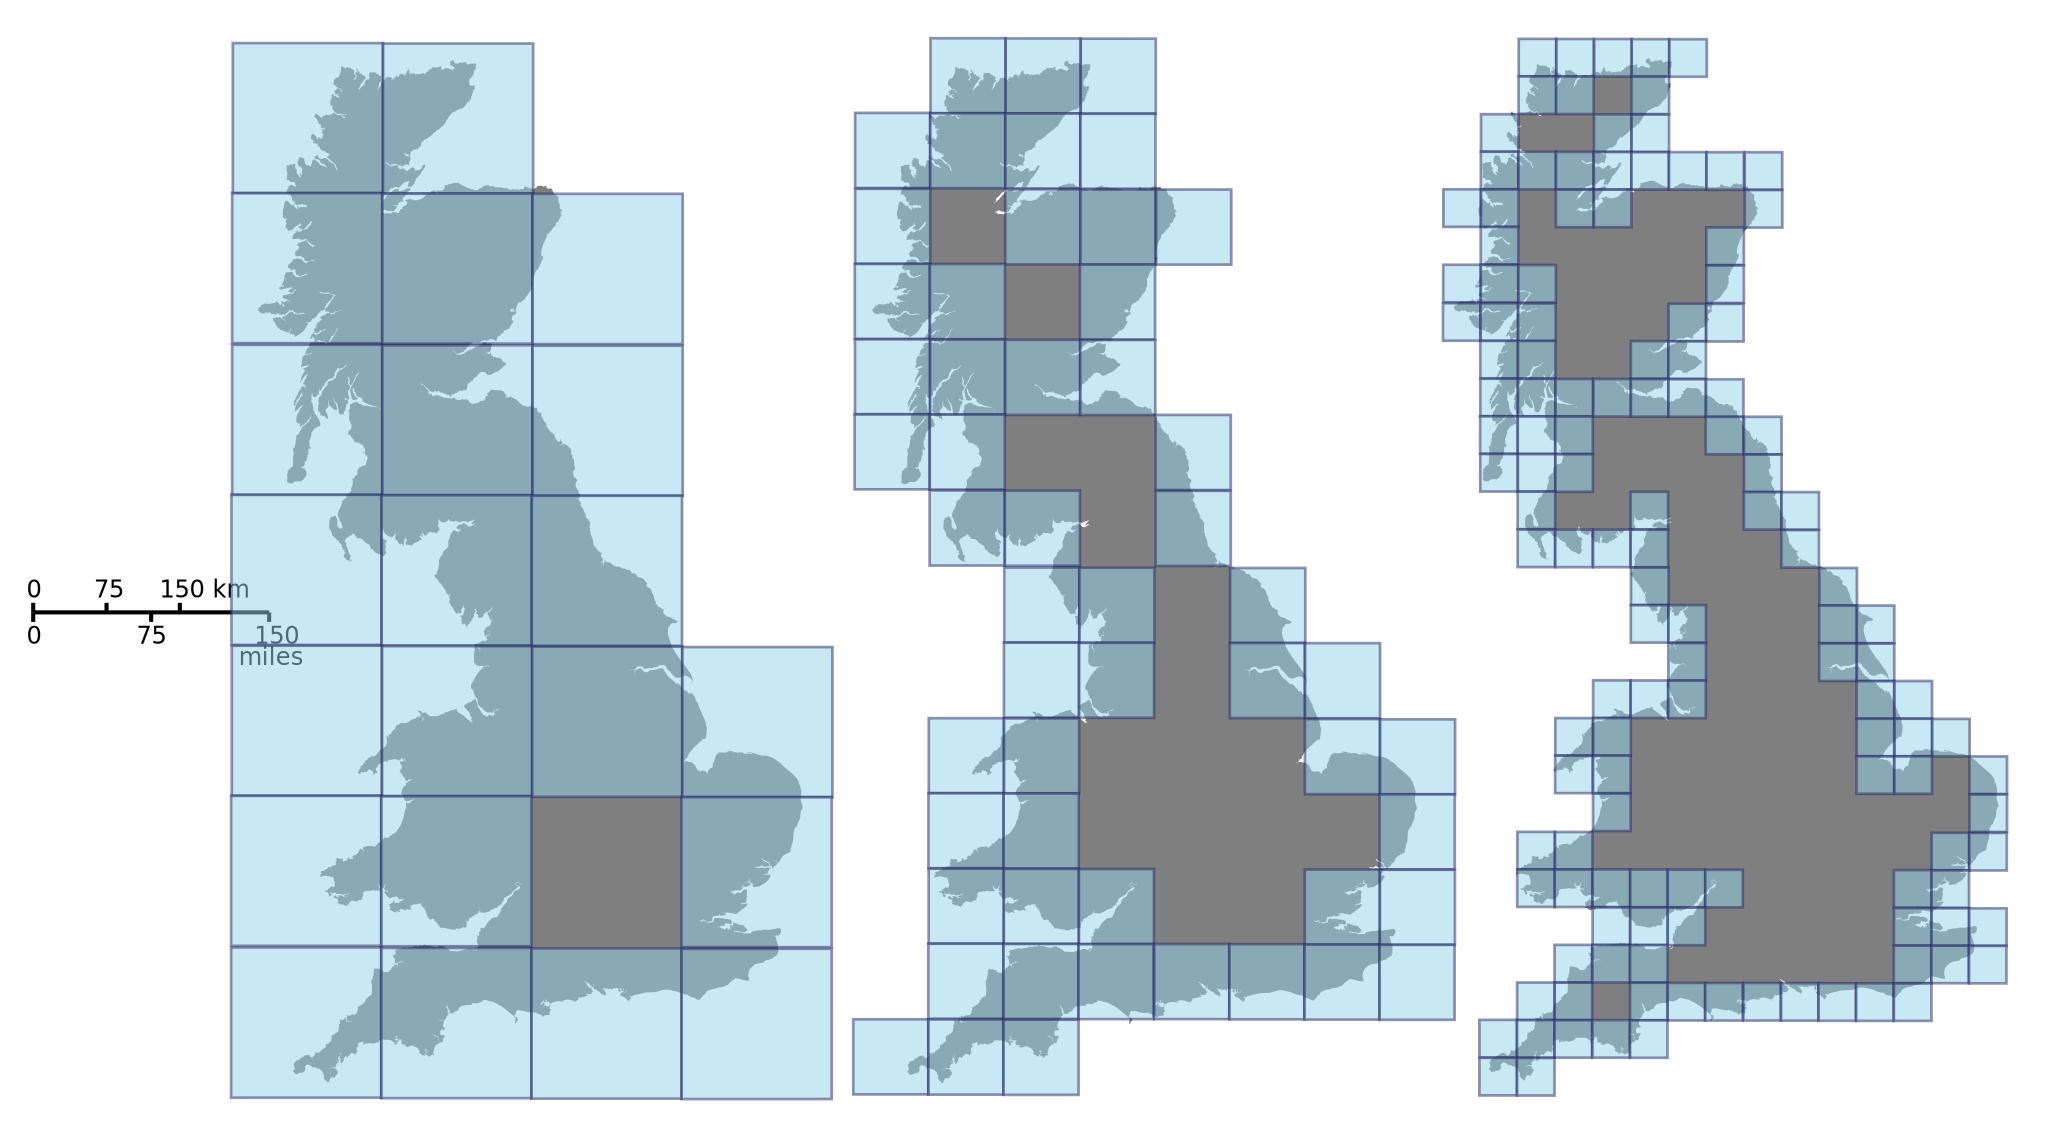
\includegraphics[width=0.7 \linewidth]{Great_Britain_Box.png}
  \caption{Box-counting method on the coastline of the Great Britain is measured to be 1.25}
  \label{fig:bc}
\end{figure}

\paragraph{The fractal parallel in music}
In this paper, inspired by the parallel between the box-counting scaling and the
hierarchical structures in music, we propose to compute a fractal-inspired
musical feature. Intuitively, the feature is computed based on the lengths of the line segments in-between the
notes. Then the feature quantifies how the lengths change with zooming-in and -out of different levels of
hierarchies in music. By construct, this feature measures and characterises
different amounts of details in musical materials. By using synthesised data and
real-world music data, we analytically demonstrate the properties of this
feature and computationally show that this feature can be useful in corpus classification and
pattern discovery. 

\paragraph{Previous work}
\subparagraph{Music Information Retrieval (MIR)}
In the research area of MIR, many
useful tools and investigation have been made to understand the hierachical
structures of music. For example, there are music musical analysis assistant \cite{hamanaka2009interactive, hamanaka2005atta}, compositional tools
\cite{hamanaka2004automatic, hamanaka2005automatic}, evaluation investigation \cite{mcfee2017evaluating, mcfee2015hierarchical} based on a variety of hierachical
structure analysis in music.
\subparagraph{Fractal methods}
Self-similarity concepts, and fractals in particular have inspired many research
in audio and music analysis \cite{bigerelle2000fractal,hsu1990fractal,hsu1991self} and composition \cite{sukumaran2009generation,leach1995nature}. In other domain of applications, the fractal theory has
been widely used in investigating time series, dynamical systems, and
non-linearity \cite{accardo1997use, higuchi1988approach}.

To the best of our
knowledge, there has not been an
attempt on computing the fractal dimensions equivalent in symbolic music by
drawing the parallel between the box-counting method and hierarchical structures
in music. 


% \paragraph{Music Information Retrieval (MIR)}
% In the research area of MIR, many
% useful tools and investigation have been made to understand the hierachical
% structures of music. For example, there are music musical analysis assistant \cite{hamanaka2009interactive, hamanaka2005atta}, compositional tools
% \cite{hamanaka2004automatic, hamanaka2005automatic}, evaluation investigation \cite{mcfee2017evaluating, mcfee2015hierarchical} based on a variety of hierachical
% structure analysis in music. To the best of our knowledge, there has not been an
% attempt on using fractal dimensions for the analysis hierarchical structures of
% music.  

%There have been also much research on how one could understand, represent and extract the
%hierachical structures automatically. A balance and feedback loop between the theories and the
%applications have stimulated much interests in the topic of hierachies in music. 

% \paragraph{Metrical structures}
% Metrical structure plays an important role in the construction and the
% perception of the hierachical structures in music. Depending on the locations of
% the musical events on the metrical grid or their relational positions to other
% notes, one can assign metrical weights/importance to the notes. The notes at more important metrical
% positions form the anchors in the hierachical structure. 

% \paragraph{musical features}
% musical features refers to summarising music events numerically. there are
% available toolbox to calculate features, such as jmir \cite{mckay2018jsymbolic}, mirtoolbox \cite{lartillot2007matlab}, the fantastic
% toolbox \cite{mullensiefen2009fantastic}. there are features such as`` note
% density per quarter note'' and ``most common melodic interval''. one can either
% take the whole piece or take a series of sliding windows and obtain a time
% series of features. using features to understand the structure of music have
% been employ in much research \cite{ren2018feature, ren153analysis,
%   bigo2018relevance}.

% \paragraph{Applications}
% Such fractal dimensions can be used as a musical feature or musical similarity in many MIR
% tasks. For example, for musical pattern discovery, we can use the fractal
% dimensions to discover repeated pattern with similar degrees of roughness in the
% melodic line. 

% Musical pattern discovery is an active subarea of MIR research. It faces many
% challenges \cite{janssen2013finding}. A music feature can characterise one certain aspect of repetition of an excerpt and therefore can be
% used in pattern discovery to retrieve partial repetitions of excerpts. 

\paragraph{Contributions}
\begin{itemize}
\item  Based on fractal geometry and the hierachical structures in music, we propose a
new feature that measures the amount of details in symbolic music.
\item  Using the proposed feature, we present a library for musical analysis and
  pattern discovery.
\item  We showcase the effectiveness of our system on various
corpora and comparing the proposed feature with other existing features of music. 
\end{itemize}

\section{The similarity dimension}
Fractals are known for the property of self-similarity. We therefore name the
new feature ``similarity dimension'' in the context of MIR, and use ``fractal
dimension'' in the original geometric context.

In this section, we describe how we compute the similarity dimension feature.

\subsection{Fractal dimensions and boxing counting}
Mathematically, the fractal dimension is defined as $$D=-\frac{logM}{logs}$$

where $M=Mass$, usually defined in terms of lengths or areas of the geometric
objects, and $s=scaling$, usually defined as how many recursive steps has been
taken in creating the fractals.

One intuition of fractal dimension is how rough or how much detail are embedded
in the geometric object. For example, the coast lines of different countries can
be measured in terms of fractal dimensions by using the box-counting method
\cite{sarkar1994efficient}, where one control the scaling factor $s$ and count
the ``boxes'' to obtain the mass $M$. Thus we can empirically compute fractal dimensions
given any geometric objects. 

\subsection{Similarity dimension in music}
In the context of music, there have been evidences that a visual-audio
correspondence exists amongst music objects \cite{thorpe2016perception}. This
can also be observed from the sheet music. Even without musical training, one can differentiate the
uneven, irregular contours of music notes against the smooth, regular contours,
and have certain expectations in the corresponding musical events. Following the
intuition given in the last paragraph, a rougher
contour which contains many details would correspond to a higher ``Mass'' in
terms of the fractal geometry.

Different measures can be defined to measure $M$, the mass of melodic contour. And
given a hierarchy of melodic reduction, we can ``zoom-in/out'' across the
hierarchy and examine have different levels of details, which can function as the scaling $s$.
Therefore, in a monophonic scenario, we can calculate a similarity dimension
using two levels in musical hierarchy using $M$ and $s$. 

In this paper, we take a simple mass measurement
$$M(n_1, n_2) = \sqrt{(t_1-t_2)^2 +(p_1-p_2)^2}$$
  where $n_i=(t_i, p_i)$, that is, a musical note is characterised by its onset time and
the pitch number. 
Intuitively, it is the line segment between two notes. By taking the sum of the
line segments, we obtain the length sum approximating the roughness of the contour
of a melodic line. 

%lengths of the holding notes and the lengths of the lines connecting the two
%notes when there is a pitch change, and 

After obtaining the mass, we can then take a ratio between different levels of
hierarchies and compute the fractal/similarity dimension. 

\begin{myhs}
\begingroup\par\noindent\advance\leftskip\mathindent\(
\begin{pboxed}\SaveRestoreHook
\column{B}{@{}>{\hspre}l<{\hspost}@{}}%
\column{E}{@{}>{\hspre}l<{\hspost}@{}}%
\>[B]{}\HSVar{dim}\HSSym{::}\HSCon{Scaling}\HSSym{\to} \HSCon{Mass}\HSSym{\to} \HSCon{Mass}\HSSym{\to} \HSCon{Double}{}\<[E]%
\\
\>[B]{}\HSVar{dim}\;\HV{\sigma}\;\HV{a_0}\;\HV{a_1}\HSSym{\mathrel{=}}\HSVar{logBase}\;\HV{\sigma}\;\HSSpecial{(}\HV{a_1}\HSSym{\mathbin{/}}\HV{a_0}\HSSpecial{)}{}\<[E]%
\ColumnHook
\end{pboxed}
\)\par\noindent\endgroup\resethooks
\end{myhs}


%The Definition of "Mass": $$M\propto{s}^{-D}$$

 \subsection{Compute the features}
 \begin{enumerate}
 \item split the music entry into m parts, n bars per part
 
 \item perform the following actions for each bar

   \begin{enumerate}
   \item  Create hierarchy:
     \begin{itemize}
     \item  take the notes in the most important positions in the bar (for example,
      in a 4/4 bar, we have a importance grid of [5,2,3,2,4,2,3,2] in the
      resolution of a quiver; so only the notes on position of the first quiver
      will be taken
      \item take the notes in the most and the second most important positions in
      the bar (we have the positions of the first and the fifth quiver in this
      case)
      \item  repeat till we consider all the importance level
      \end{itemize}
    \item Compute measurement (mass) on the hierarchy
      
      \begin{itemize}
      \item  Calculate the mass within one note: = duration in quarter length
      \item  Calculate the mass between two notes =  $\sum \sqrt{\Delta duration^2 +
        \Delta pitch^2}$ (eqv to the hypotenuse of the time and frequency
      difference)
      \item Sum up the mass (intuitively as the length of the line tracing through
      the notes in considerations)

      \end{itemize}
   \item  Take ratios and the log of the mass between the selected two hierachies: $dim = log_2(mass_{I1}/mass_{I2}) $

   \end{enumerate}
 
     
 \end{enumerate}
 
\paragraph{Interpretting the feature}
The feature consists of information from two dimensions, time and pitch. We use
a few prototipical example note combinations to illustrate how the fractal
dimensions could reflect the changes in music.

\paragraph{The similarity dimension on one piece}

\section{The Fragem package}
The implementation of the tool is in a functional programming language Haskell.

\paragraph{From modelling music using datatypes}

Model of music: [Time Signiture, [Voice]]. Because the time signiture imposes
the most common hierarchical structure in music, we use it as a default setting
for extracting hierachies to calculate the fractal dimensions. 

Model of mass: [Note] -> Maybe Double
The types give much freedom to how we could calculate the "mass". We choose the length for now for the corresponding visual contours in music. For polyphony, we can extend this to the area enclosed by two voices, and it can capture the amount of contrary motions in the piece, which is crucial for counterpoint.

Model of metrical weights: TimeSig -> [Int]
For each time signiture, we assign a list of integers of importance values to the positions of notes. Now we have a quiver as the resolution of the grid of the positions. New time signitures can be added and the resolution can be changed.

Model of computation: midi -> parameters -> [[Double], [midi]]
The input of frahem is midi files. From the parameters we introduced above, we can specify on which time scale and how many levels of hierachies we would like to analyse. The output is a time series of the fractal/self-similarity dimension. Based on the dimensions, we can also generate the patterns in the midi format with the same dimensions or up to a threshold.

Types of patterns: different types of patterns can be extracted with threshold
in the differences of fractal dimensions. 

\paragraph{Parameters}
Zoom level: 1 -> consider all notes, 2 -> consider notes with weights $>=$ 2,
...

Window size: how many bars are included in the analysis to produce one number

Sliding or hopping windows

Threshold: what is the maximum gaps between the two groups for them to be considered as belong to the same kind of pattern


\section{Experiment setting}
After computing the fractal features, we test its properties on various corpora.
\subsection{Data}
\paragraph{Individual Bars}
By varying pitch and duration in the minimalistic examples, we show how fractal
dimensions perform on a spectrum of different repetitions.

\paragraph{Synthesised Data}
Using Ionian scale, repeated interval jumps, and different amount of randomness, we check the effectiveness of the fractal dimensions. As can be computed, the fractal dimensions can indeed differentiate amongst the three different regions.
\paragraph{Hanon}
We verify the fractal dimensions are invariant under inversion, retrograde,
retrograde-inversion, chromatic transposition.

\paragraph{Bach}
Using different window length, we show the fractal dimensions are able to
combine the pitch and duration information, show the changing points in the
prelude piece.

\subsection{Correlation with known features}
We calculate the correlation between the fractal dimension with other musical
features defined in jSymbolic2. 

\subsection{Classification}
We use the synthesised data with two levels of randomness, the Hanon exercises
and Bach's fugues for the classification experiment.

Examining the heatmap, we see higher fractal dimension in the most complicated
piece, Bach's WTC. 

\subsection{Pattern discovery}
Using the MIREX dataaset, we found more patterns than the annotations.

We are extract some rhythmical patterns on not yet annotated dataset.

\section{Results}
The new fractal dimensions do not strongly correlate with features from
jSymbolic2.2. 

\section{Discussion}

Summary. 

Limitations:  

Future work:
%
%%%%%%%%%%%%%%%%%%%%%%%%
%%%%%%%%%%%%%%%%%%%%%%%%

%% Acknowledgments
%\begin{acks}                            %% acks environment is optional
                                        %% contents suppressed with 'anonymous'
  %% Commands \grantsponsor{<sponsorID>}{<name>}{<url>} and
  %% \grantnum[<url>]{<sponsorID>}{<number>} should be used to
  %% acknowledge financial support and will be used by metadata
  %% extraction tools.
%  This material is based upon work supported by the
%  \grantsponsor{GS100000001}{National Science
%    Foundation}{http://dx.doi.org/10.13039/100000001} under Grant
%  No.~\grantnum{GS100000001}{nnnnnnn} and Grant
%  No.~\grantnum{GS100000001}{mmmmmmm}.  Any opinions, findings, and
%  conclusions or recommendations expressed in this material are those
%  of the author and do not necessarily reflect the views of the
%  National Science Foundation.
%\end{acks}


%% Bibliography
\bibliography{references}


%% Appendix
%% \appendix
%% \section{Appendix}
%% 
%% %include src/appendix.lhs

\end{document}
